\documentclass[12pt]{article}

%packages
\usepackage{graphicx}
\usepackage{amsmath}
\usepackage{mathdots}
\usepackage{amsthm}
\usepackage{amssymb}
\usepackage{fancyhdr}
\usepackage{pstricks}
\usepackage{pst-node}
\pagenumbering{arabic}
\usepackage{hyperref}
\usepackage{lscape}
%Margins etc...
\setlength{\textheight}{240mm}
\setlength{\topmargin}{-17mm} \setlength{\oddsidemargin}{-4mm}
\setlength{\textwidth}{166mm} \setlength{\parindent}{0mm}
\setlength{\marginparsep}{9mm} \setlength{\parskip}{3mm}

\begin{document}
\begin{center}
\Huge{Markov Chains Exercise Sheet}\\
\tiny{Last updated: \today.}
\end{center}

\begin{enumerate}
\item Assume that a student can be in 1 of 4 states:
\begin{itemize}
	\item Rich
	\item Average
	\item Poor
	\item In Debt
\end{itemize}
Assume the following transition probabilities:

\begin{itemize}
	\item If a student is Rich, in the next time step the student will be:
	\begin{itemize}
		\item Average: .75
		\item Poor: .2
		\item In Debt: .05
	\end{itemize}
	\item If a student is Average, in the next time step the student will be:
	\begin{itemize}
		\item Rich: .05
		\item Average: .2
		\item In Debt: .45
	\end{itemize}
	\item If a student is Poor, in the next time step the student will be:
	\begin{itemize}
		\item Average: .4
		\item Poor: .3
		\item In Debt: .2
	\end{itemize}
	\item If a student is In Debt, in the next time step the student will be:
	\begin{itemize}
		\item Average: .15
		\item Poor: .3
		\item In Debt: .55
	\end{itemize}
\end{itemize}Model the above as a discrete Markov chain and:
\begin{enumerate}
	\item Draw the corresponding Markov chain and obtain the corresponding stochastic matrix.
	\item Let us assume that a student starts their studies as ``Average''. What will be the probability of them being ``Rich'' after 1,2,3 time steps?
	\item What is the steady state probability vector associated with this Markov chain?
\end{enumerate}
\item Consider the following matrices. For the matrices that are stochastic matrices, draw the associated Markov Chain and obtain the steady state probabilities (if they exist, if not, explain why).


$$\begin{array}{cccc}
\begin{pmatrix}
0&1\\
0&1\\
\end{pmatrix}
&
\begin{pmatrix}
.5&.25&.25\\
1&0&0\\
0&.23&.77\\
.8&.1&.1
\end{pmatrix}&
\begin{pmatrix}
{1\over n}&{n-1\over n}\\
{n-1\over n}&{1\over n}\\
\end{pmatrix}
&
\begin{pmatrix}
.2&.3&.5\\
.1&.1&.8\\
.7&.1&.2
\end{pmatrix}\\
\text{(a)}&\text{(b)}& \text{(c)}&\text{(d)}\\
\begin{pmatrix}
.2&.3&.1&.4\\
0&.3&.7&0\\
.5&.2&.1&.2\\
.1&0&0&.9
\end{pmatrix}&
\begin{pmatrix}
.2&.3&.5\\
.3&-.3&1\\
.2&.2&.6
\end{pmatrix}
&
\begin{pmatrix}
.5&.5&0&0\\
0&.5&.5&0\\
0&0&.5&.5\\
.5&0&0&.5\\
\end{pmatrix}
&
\begin{pmatrix}
\alpha&\beta\\
\omega&\gamma
\end{pmatrix}
\\
\text{(e)}&\text{(f)}& \text{(g)}&\text{(h)}\\
\end{array}$$

\item Consider the following (incomplete) transition matrix:

$$
\begin{pmatrix}
?&2&1.5&.5\\
?&-5&1&3\\
5&2&?&1\\
1&?&1&-2\\
\end{pmatrix}
$$
\begin{enumerate}
	\item Fill in the missing values in the transition matrix.
	\item Draw the Markov chain.
	\item Obtain the steady state probabilities.
\end{enumerate}

\item Consider the following matrices. For the matrices that are transition rate matrices, draw the associated Markov Chain and obtain the steady state probabilities (if they exist, if not, explain why).

$$\begin{array}{cccc}
\begin{pmatrix}
-1&1\\
-1&1\\
\end{pmatrix}
&
\begin{pmatrix}
-5&0&5\\
2&0&-2\\
0&3&-3\\
0&0&0
\end{pmatrix}&
\begin{pmatrix}
-3&3&0\\
0&-3&3\\
3&0&-3
\end{pmatrix}
&
\begin{pmatrix}
-a&a&0\\
b&-(a+b)&a\\
0&b&-b
\end{pmatrix}\\
\text{(a)}&\text{(b)}& \text{(c)}&\text{(d)}\\
\begin{pmatrix}
-1&1&0&0\\
0&-4&2&2\\
1&0&-2&1\\
2&0&0&-2
\end{pmatrix}&
\begin{pmatrix}
0&0&0\\
5&-10&5\\
10&0&-10
\end{pmatrix}
&
\begin{pmatrix}
-.5&.5&0&0\\
0&-.5&.5&0\\
0&0&-.5&.5\\
.5&0&0&-.5\\
\end{pmatrix}
&
\begin{pmatrix}
\alpha&\beta\\
\omega&\gamma
\end{pmatrix}
\\
\text{(e)}&\text{(f)}& \text{(g)}&\text{(h)}\\
\end{array}$$


\item Consider the following continuous Markov chain.

\begin{center}
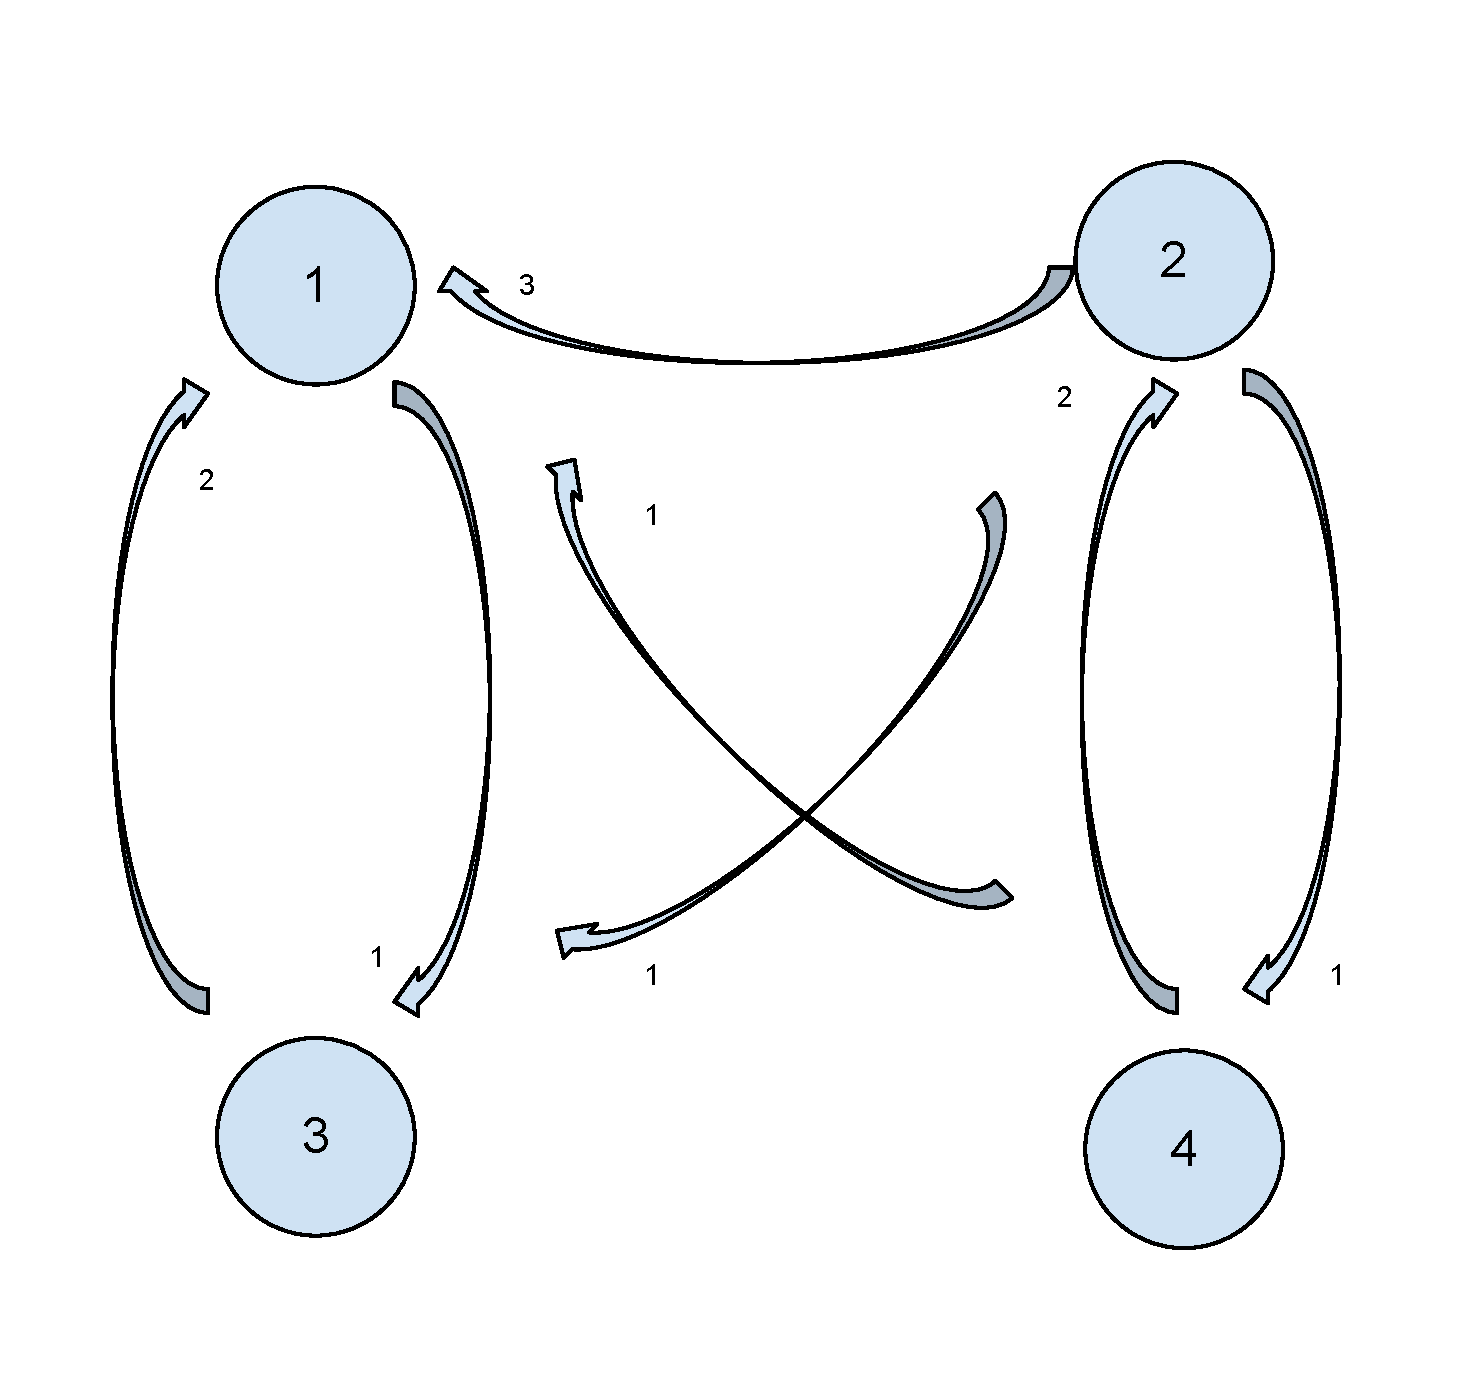
\includegraphics[width=8cm]{Markov_Chains_Ex_5.pdf}
\end{center}

\begin{enumerate}
	\item Obtain the transition rate matrix.
	\item Obtain the steady state probabilities for this Markov chain.
	\item Obtain the corresponding discrete time Markov chain.
	\item Draw the corresponding Markov chain.
	\item Obtain the steady state probabilities for the discretized Markov chain.
\end{enumerate}

\end{enumerate}

\end{document}
